\documentclass{article}
\usepackage[utf8]{inputenc}
\usepackage[spanish]{babel}
\usepackage{enumerate} % enumerados
\usepackage{graphicx}
\usepackage{hyperref}
\usepackage{minted}

\title{Práctica N° 17 - FdLP}
\author{Christian Omar Rodriguez Huamanñahui\\
crodriguezh@ulasalle.edu.pe}
\date{NOV 2022}

\maketitle
\clearpage
\usepackage[margin=0.5in]{geometry}
\begin{document}
\documentclass

\tableofcontents
\clearpage

\section{Ejercicio 1}
\begin{figure}[h]
\centering
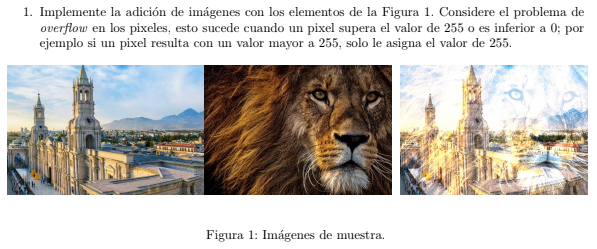
\includegraphics[scale=1]{EJ1.png}
\end{figure}
\\

- CÓDIGO EN GOLANG (CONCURRENCIA Y PARALELISMO):
\begin{minted}{go}
// --------EJERCICIO1: CONCURRENCIA Y PARALELISMO--------
// IMPORTANDO LIBRERIAS NECESARIAS
package main

import (
	"fmt"
	"image"
	"image/color"
	"image/jpeg"
	"log"
	"os"
	"path/filepath"
	"strings"
	"sync"
	"time"
)

func main() {
	//VARIABLE DEL FADE (BRILLO) ENTRE IMÁGENES
	FADE := 0.75
	//SE REGISTRA LA RUTA DE LA PRIMERA IMÁGEN
	IMPORTAR_IMAGEN1 := "src/OG/AFTER_HOURS.jpg"
	f, err := os.Open(IMPORTAR_IMAGEN1)
	check(err)

	//SE CAPTURAN LOS VALORES DE LA 1RA IMAGEN
	img, _, err := image.Decode(f)

	//SE REGISTRA LA RUTA DE LA SEGUNDA IMÁGEN
	IMPORTAR_IMAGEN2 := "src/OG/DAWN_FM.jpg"
	f2, err2 := os.Open(IMPORTAR_IMAGEN2)
	check(err2)

	//SE CAPTURAN LOS VALORES DE LA 2DA IMAGEN
	img2, _, err := image.Decode(f2)

	//SE RECONOCE EL TAMAÑO DE CADA IMAGEN
	TAMAÑO := img.Bounds().Size()
	rect := image.Rect(0, 0, TAMAÑO.X, TAMAÑO.Y)
	wImg := image.NewRGBA(rect)

	//GOROUTINE
	wg := new(sync.WaitGroup)

	//TEMPORIZADOR: INICIAR
	start := time.Now()

	//CICLO QUE RECORRE TODO Y (ALTO)
	for ALTO := 0; ALTO < TAMAÑO.Y; ALTO++ {

		//GOROUTINE
		wg.Add(1)
		ALTO := ALTO
		go func() {

			// CICLO QUE RECORRE TODO X (ANCHO)
			for ANCHO := 0; ANCHO < TAMAÑO.X; ANCHO++ {
				pixel := img.At(ANCHO, ALTO)
				pixel2 := img2.At(ANCHO, ALTO)

				OG_COLOR1 := color.RGBAModel.Convert(pixel).(color.RGBA)
				OG_COLOR2 := color.RGBAModel.Convert(pixel2).(color.RGBA)

				// CONVIRTIENDO ANÁLISIS RGB A VALORES FLOAT (IMÁGEN 1 Y 2)
				RED_CHANNEL := float64(OG_COLOR1.R)
				GREEN_CHANNEL := float64(OG_COLOR1.G)
				BLUE_CHANNEL := float64(OG_COLOR1.B)

				RED_CHANNEL2 := float64(OG_COLOR2.R)
				GREEN_CHANNEL2 := float64(OG_COLOR2.G)
				BLUE_CHANNEL2 := float64(OG_COLOR2.B)

				// COMBINANDO VALORES RGB DE AMBAS IMÁGENES
				RED_CHANNEL3 := uint8((RED_CHANNEL + RED_CHANNEL2) * FADE)
				GREEN_CHANNEL3 := uint8((GREEN_CHANNEL + GREEN_CHANNEL2) * FADE)
				BLUE_CHANNEL3 := uint8((BLUE_CHANNEL + BLUE_CHANNEL2) * FADE)

				//ASIGNANDO VALOR MÁXIMO DE CANT. DE PIXELES POR CADA CANAL DE LA IMÁGEN 3
				if RED_CHANNEL3 > 255 || GREEN_CHANNEL3 > 255 || BLUE_CHANNEL3 > 255 {
					RED_CHANNEL3 = 255
					GREEN_CHANNEL3 = 255
					BLUE_CHANNEL3 = 255
				}
				if RED_CHANNEL3 < 0 || GREEN_CHANNEL3 < 0 || BLUE_CHANNEL3 < 0 {
					RED_CHANNEL3 = 0
					GREEN_CHANNEL3 = 0
					BLUE_CHANNEL3 = 0
				}

				//SETTEANDO LOS VALORES RGBA DE CADA CANAL
				COLOR := color.RGBA{
					R: RED_CHANNEL3, G: GREEN_CHANNEL3, B: BLUE_CHANNEL3, A: OG_COLOR1.A,
				}
				wImg.Set(ANCHO, ALTO, COLOR)
			}
			defer wg.Done()
		}()
	}
	wg.Wait()

	//FINALIZAR CRONÓMETRO E IMPRIMIR EL TIEMPO
	elapsed := time.Since(start)
	print("Se guardó correctamente la nueva imágen en la carpeta: 'OUTPUT'")
	log.Printf("\nTIEMPO | EJERCICIO1 | GOROUTINE: %s", elapsed)

	//DETERMINANDO CARPETA DONDE SE GUARDARÁ EL RESULTADO
	imgOut := "src/OUT/"

	//CREAR EL RESULTADO
	ext := filepath.Ext(IMPORTAR_IMAGEN1)
	name := strings.TrimSuffix(filepath.Base("OUTPUT"), ext)
	newImagePath := fmt.Sprintf("%s/%s_CONCURRENCIA-EJ1%s", filepath.Dir(imgOut), name, ext)
	fg, err := os.Create(newImagePath)
	defer fg.Close()
	check(err)
	err = jpeg.Encode(fg, wImg, nil)
	check(err)
}

// POR SI HAY ERRORES
func check(err error) {
	if err != nil {
		panic(err)
	}
}
\end{minted}

- CÓDIGO EN GOLANG (SECUENCIAL):
\begin{minted}{go}
// --------EJERCICIO1: SECUENCIAL--------
// IMPORTANDO LIBRERIAS NECESARIAS
package main

import (
	"fmt"
	"image"
	"image/color"
	"image/jpeg"
	"log"
	"os"
	"path/filepath"
	"strings"
	"time"
)

func main() {
	//VARIABLE DEL FADE (BRILLO) ENTRE IMÁGENES
	FADE := 0.75
	//SE REGISTRA LA RUTA DE LA PRIMERA IMÁGEN
	IMPORTAR_IMAGEN1 := "src/OG/AFTER_HOURS.jpg"
	f, err := os.Open(IMPORTAR_IMAGEN1)
	check(err)

	//SE CAPTURAN LOS VALORES DE LA 1RA IMAGEN
	img, _, err := image.Decode(f)

	//SE REGISTRA LA RUTA DE LA SEGUNDA IMÁGEN
	IMPORTAR_IMAGEN2 := "src/OG/DAWN_FM.jpg"
	f2, err2 := os.Open(IMPORTAR_IMAGEN2)
	check(err2)

	//SE CAPTURAN LOS VALORES DE LA 2DA IMAGEN
	img2, _, err := image.Decode(f2)

	//SE RECONOCE EL TAMAÑO DE CADA IMAGEN
	TAMAÑO := img.Bounds().Size()
	rect := image.Rect(0, 0, TAMAÑO.X, TAMAÑO.Y)
	wImg := image.NewRGBA(rect)

	//TEMPORIZADOR: INICIAR
	start := time.Now()
	//CICLO QUE RECORRE TODO Y (ALTO)
	for ALTO := 0; ALTO < TAMAÑO.Y; ALTO++ {
		// CICLO QUE RECORRE TODO X (ANCHO)
		for ANCHO := 0; ANCHO < TAMAÑO.X; ANCHO++ {
			pixel := img.At(ANCHO, ALTO)
			pixel2 := img2.At(ANCHO, ALTO)

			OG_COLOR1 := color.RGBAModel.Convert(pixel).(color.RGBA)
			OG_COLOR2 := color.RGBAModel.Convert(pixel2).(color.RGBA)

			// CONVIRTIENDO ANÁLISIS RGB A VALORES FLOAT (IMÁGEN 1 Y 2)
			RED_CHANNEL := float64(OG_COLOR1.R)
			GREEN_CHANNEL := float64(OG_COLOR1.G)
			BLUE_CHANNEL := float64(OG_COLOR1.B)

			RED_CHANNEL2 := float64(OG_COLOR2.R)
			GREEN_CHANNEL2 := float64(OG_COLOR2.G)
			BLUE_CHANNEL2 := float64(OG_COLOR2.B)

			// COMBINANDO VALORES RGB DE AMBAS IMÁGENES
			RED_CHANNEL3 := uint8((RED_CHANNEL + RED_CHANNEL2) * FADE)
			GREEN_CHANNEL3 := uint8((GREEN_CHANNEL + GREEN_CHANNEL2) * FADE)
			BLUE_CHANNEL3 := uint8((BLUE_CHANNEL + BLUE_CHANNEL2) * FADE)

			//ASIGNANDO VALOR MÁXIMO DE CANT. DE PIXELES POR CADA CANAL DE LA IMÁGEN 3
			if RED_CHANNEL3 > 255 || GREEN_CHANNEL3 > 255 || BLUE_CHANNEL3 > 255 {
				RED_CHANNEL3 = 255
				GREEN_CHANNEL3 = 255
				BLUE_CHANNEL3 = 255
			}
			if RED_CHANNEL3 < 0 || GREEN_CHANNEL3 < 0 || BLUE_CHANNEL3 < 0 {
				RED_CHANNEL3 = 0
				GREEN_CHANNEL3 = 0
				BLUE_CHANNEL3 = 0
			}

			//SETTEANDO LOS VALORES RGBA DE CADA CANAL
			COLOR := color.RGBA{
				R: RED_CHANNEL3, G: GREEN_CHANNEL3, B: BLUE_CHANNEL3, A: OG_COLOR1.A,
			}
			wImg.Set(ANCHO, ALTO, COLOR)
		}
	}

	//FINALIZAR CRONÓMETRO E IMPRIMIR EL TIEMPO
	elapsed := time.Since(start)
	print("Se guardó correctamente la nueva imágen en la carpeta: 'OUTPUT'")
	log.Printf("\nTIEMPO | EJERCICIO1 | SECUENCIAL: %s", elapsed)

	//DETERMINANDO CARPETA DONDE SE GUARDARÁ EL RESULTADO
	imgOut := "src/OUT/"

	//CREAR EL RESULTADO
	ext := filepath.Ext(IMPORTAR_IMAGEN1)
	name := strings.TrimSuffix(filepath.Base("OUTPUT"), ext)
	newImagePath := fmt.Sprintf("%s/%s_SECUENCIAL-EJ1%s", filepath.Dir(imgOut), name, ext)
	fg, err := os.Create(newImagePath)
	defer fg.Close()
	check(err)
	err = jpeg.Encode(fg, wImg, nil)
	check(err)
}

// POR SI HAY ERRORES
func check(err error) {
	if err != nil {
		panic(err)
	}
}

\end{minted}

\\
- CONCURRENCIA Y PARALELISTMO: EJECUCIÓN Y TIEMPO EN CONSOLA (ADMIN/POWERSHELL):
\begin{figure}[h]
\centering
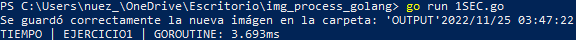
\includegraphics[scale=1]{CON1.png}
\end{figure}
\\
- SECUENCIAL: EJECUCIÓN Y TIEMPO EN CONSOLA (ADMIN/POWERSHELL):
\begin{figure}[h]
\centering
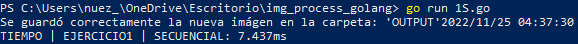
\includegraphics[scale=1]{SEC1.png}
\end{figure}
\\
- INPUT DE IMÁGENES (ARCHIVOS: "AFTER HOURS" Y "DAWN FM"):
\begin{figure}[h]
\centering
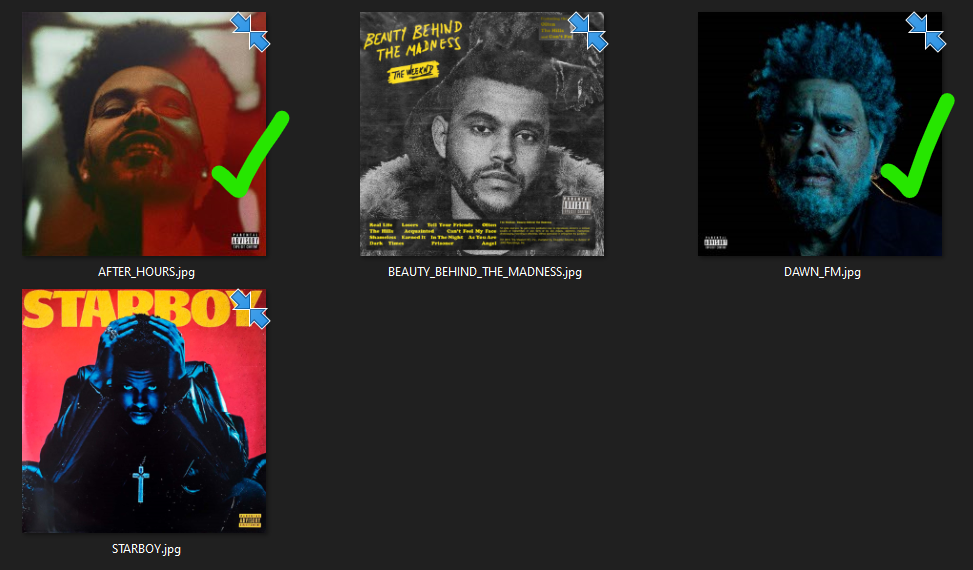
\includegraphics[scale=0.4]{IMG1.png}
\end{figure}
\\
\newpage
- OUTPUT DE IMAGEN RESULTANTE:
\begin{figure}[h]
\centering
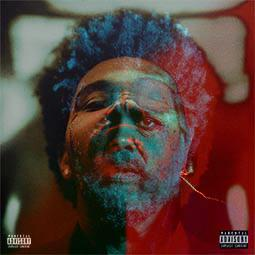
\includegraphics[scale=1]{OUTPUT_CONCURRENCIA-EJ1.jpg}
\end{figure}
\newpage

\section{Ejercicio 2}
\begin{figure}[h]
\centering
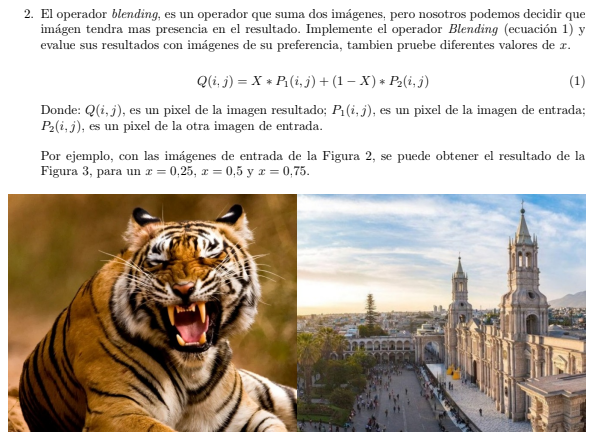
\includegraphics[scale=1]{EJ2A.png}
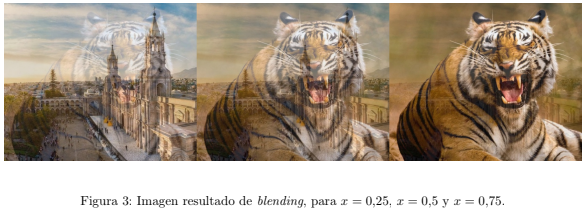
\includegraphics[scale=1]{EJ2B.png}
\end{figure}
- CÓDIGO EN GOLANG (CONCURRENCIA Y PARALELISMO):
\begin{minted}{go}
// --------EJERCICIO2: CONCURRENCIA Y PARALELISMO--------
// IMPORTANDO LIBRERIAS NECESARIAS
package main

import (
	"fmt"
	"image"
	"image/color"
	"image/jpeg"
	"log"
	"os"
	"path/filepath"
	"strings"
	"sync"
	"time"
)

func main() {
	//VARIABLE DEL FADE (BRILLO) ENTRE IMÁGENES / VALORES ENTRE 0 - 1 (PROBAR: 0.25 - 0.50 - 0.75)
	FADE := 0.75
	//SE REGISTRA LA RUTA DE LA PRIMERA IMÁGEN
	IMPORTAR_IMAGEN1 := "src/OG/BEAUTY_BEHIND_THE_MADNESS.jpg"
	f, err := os.Open(IMPORTAR_IMAGEN1)
	check(err)

	//SE CAPTURAN LOS VALORES DE LA 1RA IMAGEN
	img, _, err := image.Decode(f)

	//SE REGISTRA LA RUTA DE LA SEGUNDA IMÁGEN
	IMPORTAR_IMAGEN2 := "src/OG/STARBOY.jpg"
	f2, err2 := os.Open(IMPORTAR_IMAGEN2)
	check(err2)

	//SE CAPTURAN LOS VALORES DE LA 2DA IMAGEN
	img2, _, err := image.Decode(f2)

	//SE RECONOCE EL TAMAÑO DE CADA IMAGEN
	TAMAÑO := img.Bounds().Size()
	rect := image.Rect(0, 0, TAMAÑO.X, TAMAÑO.Y)
	wImg := image.NewRGBA(rect)

	//GOROUTINE
	wg := new(sync.WaitGroup)

	//TEMPORIZADOR: INICIAR
	start := time.Now()

	//CICLO QUE RECORRE TODO Y (ALTO)
	for ALTO := 0; ALTO < TAMAÑO.Y; ALTO++ {

		//GOROUTINE
		wg.Add(1)
		ALTO := ALTO
		go func() {

			// CICLO QUE RECORRE TODO X (ANCHO)
			for ANCHO := 0; ANCHO < TAMAÑO.X; ANCHO++ {
				pixel := img.At(ANCHO, ALTO)
				pixel2 := img2.At(ANCHO, ALTO)

				OG_COLOR1 := color.RGBAModel.Convert(pixel).(color.RGBA)
				OG_COLOR2 := color.RGBAModel.Convert(pixel2).(color.RGBA)

				// CONVIRTIENDO ANÁLISIS RGB A VALORES FLOAT (IMÁGEN 1 Y 2)
				RED_CHANNEL := float64(OG_COLOR1.R)
				GREEN_CHANNEL := float64(OG_COLOR1.G)
				BLUE_CHANNEL := float64(OG_COLOR1.B)

				RED_CHANNEL2 := float64(OG_COLOR2.R)
				GREEN_CHANNEL2 := float64(OG_COLOR2.G)
				BLUE_CHANNEL2 := float64(OG_COLOR2.B)

				// REALIZANDO MEZCLA FADE CON LA FÓRMULA ESTABLECIDA EN EL EJERCICIO2
				RED_CHANNEL3 := uint8(FADE*RED_CHANNEL + (1-FADE)*RED_CHANNEL2)
				GREEN_CHANNEL3 := uint8(FADE*GREEN_CHANNEL + (1-FADE)*GREEN_CHANNEL2)
				BLUE_CHANNEL3 := uint8(FADE*BLUE_CHANNEL + (1-FADE)*BLUE_CHANNEL2)
				COLOR := color.RGBA{
					R: RED_CHANNEL3, G: GREEN_CHANNEL3, B: BLUE_CHANNEL3, A: OG_COLOR1.A,
				}
				wImg.Set(ANCHO, ALTO, COLOR)
			}
			defer wg.Done()
		}()
	}
	wg.Wait()

	//FINALIZAR CRONÓMETRO E IMPRIMIR EL TIEMPO
	elapsed := time.Since(start)
	print("Se guardó correctamente la nueva imágen en la carpeta: 'OUTPUT'")
	log.Printf("\nTIEMPO | EJERCICIO2 | GOROUTINE: %s", elapsed)

	//DETERMINANDO CARPETA DONDE SE GUARDARÁ EL RESULTADO
	imgOut := "src/OUT/"

	//CREAR EL RESULTADO
	ext := filepath.Ext(IMPORTAR_IMAGEN1)
	name := strings.TrimSuffix(filepath.Base("OUTPUT"), ext)
	newImagePath := fmt.Sprintf("%s/%s_CONCURRENCIA-EJ2%s", filepath.Dir(imgOut), name, ext)
	fg, err := os.Create(newImagePath)
	defer fg.Close()
	check(err)
	err = jpeg.Encode(fg, wImg, nil)
	check(err)
}

// POR SI HAY ERRORES
func check(err error) {
	if err != nil {
		panic(err)
	}
}
\end{minted}
\\
- CÓDIGO EN GOLANG (SECUENCIAL):
\begin{minted}{go}
// --------EJERCICIO2: SECUENCIAL--------
// IMPORTANDO LIBRERIAS NECESARIAS
package main

import (
	"fmt"
	"image"
	"image/color"
	"image/jpeg"
	"log"
	"os"
	"path/filepath"
	"strings"
	"time"
)

func main() {
	//VARIABLE DEL FADE (BRILLO) ENTRE IMÁGENES / VALORES ENTRE 0 - 1 (PROBAR: 0.25 - 0.50 - 0.75)
	FADE := 0.25
	//SE REGISTRA LA RUTA DE LA PRIMERA IMÁGEN
	IMPORTAR_IMAGEN1 := "src/OG/BEAUTY_BEHIND_THE_MADNESS.jpg"
	f, err := os.Open(IMPORTAR_IMAGEN1)
	check(err)

	//SE CAPTURAN LOS VALORES DE LA 1RA IMAGEN
	img, _, err := image.Decode(f)

	//SE REGISTRA LA RUTA DE LA SEGUNDA IMÁGEN
	IMPORTAR_IMAGEN2 := "src/OG/STARBOY.jpg"
	f2, err2 := os.Open(IMPORTAR_IMAGEN2)
	check(err2)

	//SE CAPTURAN LOS VALORES DE LA 2DA IMAGEN
	img2, _, err := image.Decode(f2)

	//SE RECONOCE EL TAMAÑO DE CADA IMAGEN
	TAMAÑO := img.Bounds().Size()
	rect := image.Rect(0, 0, TAMAÑO.X, TAMAÑO.Y)
	wImg := image.NewRGBA(rect)

	start := time.Now()
	// loop though all the x

	for ALTO := 0; ALTO < TAMAÑO.Y; ALTO++ {
		for ANCHO := 0; ANCHO < TAMAÑO.X; ANCHO++ {
			pixel := img.At(ANCHO, ALTO)
			pixel2 := img2.At(ANCHO, ALTO)

			OG_COLOR1 := color.RGBAModel.Convert(pixel).(color.RGBA)
			OG_COLOR2 := color.RGBAModel.Convert(pixel2).(color.RGBA)

			// CONVIRTIENDO ANÁLISIS RGB A VALORES FLOAT (IMÁGEN 1 Y 2)
			RED_CHANNEL := float64(OG_COLOR1.R)
			GREEN_CHANNEL := float64(OG_COLOR1.G)
			BLUE_CHANNEL := float64(OG_COLOR1.B)

			RED_CHANNEL2 := float64(OG_COLOR2.R)
			GREEN_CHANNEL2 := float64(OG_COLOR2.G)
			BLUE_CHANNEL2 := float64(OG_COLOR2.B)

			// REALIZANDO MEZCLA FADE CON LA FÓRMULA ESTABLECIDA EN EL EJERCICIO2
			RED_CHANNEL3 := uint8(FADE*RED_CHANNEL + (1-FADE)*RED_CHANNEL2)
			GREEN_CHANNEL3 := uint8(FADE*GREEN_CHANNEL + (1-FADE)*GREEN_CHANNEL2)
			BLUE_CHANNEL3 := uint8(FADE*BLUE_CHANNEL + (1-FADE)*BLUE_CHANNEL2)
			COLOR := color.RGBA{
				R: RED_CHANNEL3, G: GREEN_CHANNEL3, B: BLUE_CHANNEL3, A: OG_COLOR1.A,
			}
			wImg.Set(ANCHO, ALTO, COLOR)
		}
	}

	//FINALIZAR CRONÓMETRO E IMPRIMIR EL TIEMPO
	elapsed := time.Since(start)
	print("Se guardó correctamente la nueva imágen en la carpeta: 'OUTPUT'")
	log.Printf("\nTIEMPO | EJERCICIO2 | SECUENCIAL: %s", elapsed)

	//DETERMINANDO CARPETA DONDE SE GUARDARÁ EL RESULTADO
	imgOut := "src/OUT/"

	//CREAR EL RESULTADO
	ext := filepath.Ext(IMPORTAR_IMAGEN1)
	name := strings.TrimSuffix(filepath.Base("OUTPUT"), ext)
	newImagePath := fmt.Sprintf("%s/%s_SECUENCIAL-EJ2%s", filepath.Dir(imgOut), name, ext)
	fg, err := os.Create(newImagePath)
	defer fg.Close()
	check(err)
	err = jpeg.Encode(fg, wImg, nil)
	check(err)
}

// POR SI HAY ERRORES
func check(err error) {
	if err != nil {
		panic(err)
	}
}

\end{minted}

\\
- CONCURRENCIA Y PARALELISTMO: EJECUCIÓN Y TIEMPO EN CONSOLA (ADMIN/POWERSHELL):
\begin{figure}[h]
\centering
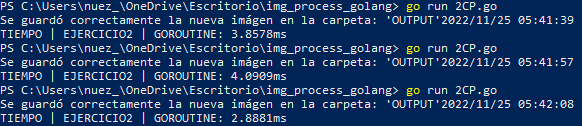
\includegraphics[scale=1]{CON2.png}
\end{figure}
\\
- SECUENCIAL: EJECUCIÓN Y TIEMPO EN CONSOLA (ADMIN/POWERSHELL):
\begin{figure}[h]
\centering
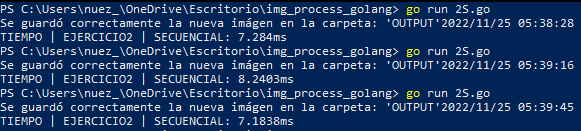
\includegraphics[scale=1]{SEC2.png}
\end{figure}
\\
- INPUT DE IMÁGENES (ARCHIVOS: "BEAUTY BEHIND THE MADNESS" Y "STARBOY"):
\begin{figure}[h]
\centering
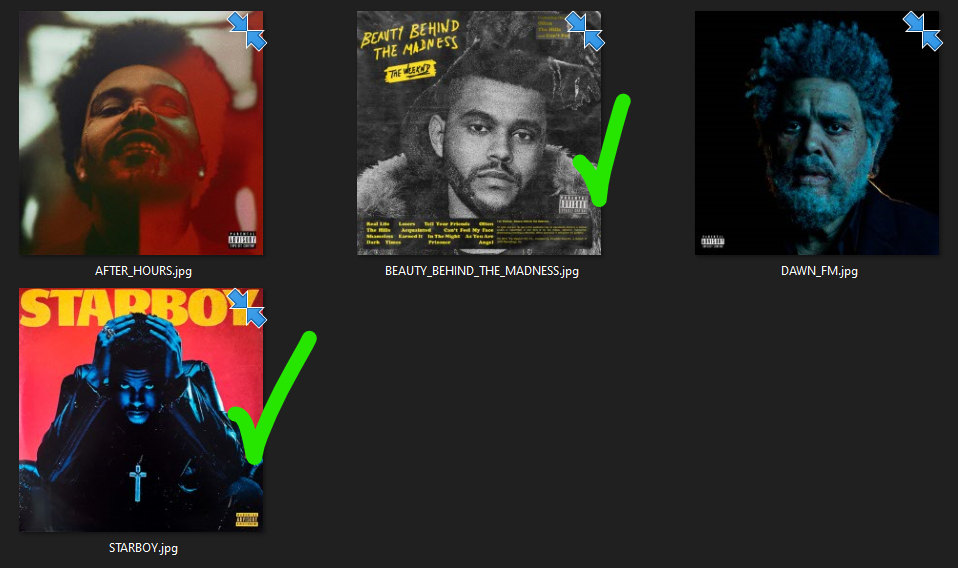
\includegraphics[scale=0.4]{IMG2.png}
\end{figure}
\\
\newpage
- OUTPUT DE IMAGEN RESULTANTE:
\begin{figure}[h]
\centering
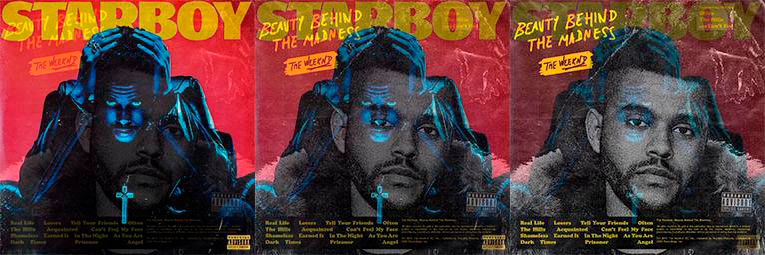
\includegraphics[scale=1]{RES2.png}
\end{figure}
\newpage

\section{Ejercicio 3}
\begin{figure}[h]
\centering
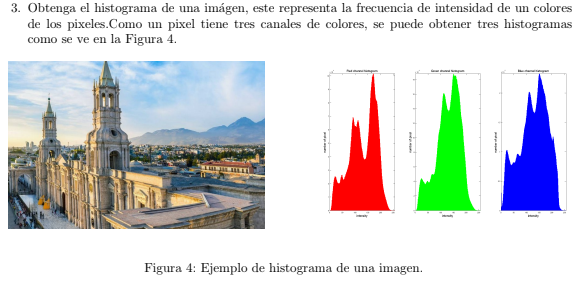
\includegraphics[scale=1]{EJ3.png}
\end{figure}
- CÓDIGO EN GOLANG (CONCURRENCIA Y PARALELISMO):
\begin{minted}{go}
// --------EJERCICIO3: CONCURRENCIA Y PARALELISMO--------
// IMPORTANDO LIBRERIAS NECESARIAS
package main

import (
	"fmt"
	"image"
	"image/color"
	"image/jpeg"
	"log"
	"os"
	"path/filepath"
	"strings"
	"sync"
	"time"
)

func main() {

	txt, err := os.Create("CANAL_ROJO.txt")
	if err != nil {
		fmt.Printf("error", err)
		return
	}
	txt1, err := os.Create("CANAL_VERDE.txt")
	if err != nil {
		fmt.Printf("error", err)
		return
	}
	txt2, err := os.Create("CANAL_AZUL.txt")
	if err != nil {
		fmt.Printf("error", err)
		return
	}
	//VARIABLE DEL FADE (BRILLO) ENTRE IMÁGENES / VALORES ENTRE 0 - 1 (PROBAR: 0.25 - 0.50 - 0.75)
	//SE REGISTRA LA RUTA DE LA PRIMERA IMÁGEN
	IMPORTAR_IMAGEN1 := "src/OG/ASTROWORLD.jpg"
	f, err := os.Open(IMPORTAR_IMAGEN1)
	check(err)

	//SE CAPTURAN LOS VALORES DE LA IMAGEN
	img, _, err := image.Decode(f)

	TAMAÑO := img.Bounds().Size()
	rect := image.Rect(0, 0, TAMAÑO.X, TAMAÑO.Y)
	wImg := image.NewRGBA(rect)

	//GOROUTINE
	wg := new(sync.WaitGroup)

	//TEMPORIZADOR: INICIAR
	start := time.Now()

	//CICLO QUE RECORRE TODO Y (ALTO)
	for ALTO := 0; ALTO < TAMAÑO.Y; ALTO++ {

		//GOROUTINE
		wg.Add(1)
		ALTO := ALTO
		go func() {

			// CICLO QUE RECORRE TODO X (ANCHO)
			for ANCHO := 0; ANCHO < TAMAÑO.X; ANCHO++ {
				pixel := img.At(ANCHO, ALTO)
				OG_COLOR := color.RGBAModel.Convert(pixel).(color.RGBA)

				// CONVIRTIENDO ANÁLISIS RGB A VALORES FLOAT (IMÁGEN 1 Y 2)
				RED_CHANNEL := float64(OG_COLOR.R)
				GREEN_CHANNEL := float64(OG_COLOR.G)
				BLUE_CHANNEL := float64(OG_COLOR.B)

				_, err = txt.WriteString(fmt.Sprintf("%d\n", uint8(RED_CHANNEL)))
				if err != nil {
					fmt.Printf("error", err)
				}
				_, err = txt1.WriteString(fmt.Sprintf("%d\n", uint8(GREEN_CHANNEL)))
				if err != nil {
					fmt.Printf("error", err)
				}
				_, err = txt2.WriteString(fmt.Sprintf("%d\n", uint8(BLUE_CHANNEL)))
				if err != nil {
					fmt.Printf("error", err)
				}
			}
			defer wg.Done()
		}()
	}
	wg.Wait()

	//FINALIZAR CRONÓMETRO E IMPRIMIR EL TIEMPO
	elapsed := time.Since(start)
	print("Se guardaron correctamente los txt con información de cada canal RGB en la carpeta: 'OUTPUT'")
	log.Printf("\nTIEMPO | EJERCICIO3 | GOROUTINE: %s", elapsed)

	//DETERMINANDO CARPETA DONDE SE GUARDARÁ EL RESULTADO
	imgOut := "src/OUT/"

	//CREAR EL RESULTADO
	ext := filepath.Ext(IMPORTAR_IMAGEN1)
	name := strings.TrimSuffix(filepath.Base("OUTPUT"), ext)
	newImagePath := fmt.Sprintf("%s/%s_CONCURRENCIA-EJ3%s", filepath.Dir(imgOut), name, ext)
	fg, err := os.Create(newImagePath)
	defer fg.Close()
	check(err)
	err = jpeg.Encode(fg, wImg, nil)
	check(err)
}

// POR SI HAY ERRORES
func check(err error) {
	if err != nil {
		panic(err)
	}
}

\end{minted}
\\
- CÓDIGO EN GOLANG (SECUENCIAL):
\begin{minted}{go}
// --------EJERCICIO3: SECUENCIAL--------
// IMPORTANDO LIBRERIAS NECESARIAS
package main

import (
	"fmt"
	"image"
	"image/color"
	"image/jpeg"
	"log"
	"os"
	"path/filepath"
	"strings"
	"time"
)

func main() {
	ROJO, err := os.Create("CANAL_ROJO.txt")
	if err != nil {
		fmt.Printf("error", err)
		return
	}
	VERDE, err := os.Create("CANAL_VERDE.txt")
	if err != nil {
		fmt.Printf("error", err)
		return
	}
	AZUL, err := os.Create("CANAL_AZUL.txt")
	if err != nil {
		fmt.Printf("error", err)
		return
	}
	//VARIABLE DEL FADE (BRILLO) ENTRE IMÁGENES / VALORES ENTRE 0 - 1 (PROBAR: 0.25 - 0.50 - 0.75)
	//SE REGISTRA LA RUTA DE LA PRIMERA IMÁGEN
	IMPORTAR_IMAGEN1 := "src/OG/ASTROWORLD.jpg"
	f, err := os.Open(IMPORTAR_IMAGEN1)
	check(err)

	//SE CAPTURAN LOS VALORES DE LA IMAGEN
	img, _, err := image.Decode(f)

	TAMAÑO := img.Bounds().Size()
	rect := image.Rect(0, 0, TAMAÑO.X, TAMAÑO.Y)
	wImg := image.NewRGBA(rect)

	//TEMPORIZADOR: INICIAR
	start := time.Now()

	//CICLO QUE RECORRE TODO Y (ALTO)
	for ALTO := 0; ALTO < TAMAÑO.Y; ALTO++ {
		// CICLO QUE RECORRE TODO X (ANCHO)
		for ANCHO := 0; ANCHO < TAMAÑO.X; ANCHO++ {
			pixel := img.At(ANCHO, ALTO)
			OG_COLOR := color.RGBAModel.Convert(pixel).(color.RGBA)

			// CONVIRTIENDO ANÁLISIS RGB A VALORES FLOAT (IMÁGEN 1 Y 2)
			RED_CHANNEL := float64(OG_COLOR.R)
			GREEN_CHANNEL := float64(OG_COLOR.G)
			BLUE_CHANNEL := float64(OG_COLOR.B)

			_, err = ROJO.WriteString(fmt.Sprintf("%d\n", uint8(RED_CHANNEL)))
			if err != nil {
				fmt.Printf("error", err)
			}
			_, err = VERDE.WriteString(fmt.Sprintf("%d\n", uint8(GREEN_CHANNEL)))
			if err != nil {
				fmt.Printf("error", err)
			}
			_, err = AZUL.WriteString(fmt.Sprintf("%d\n", uint8(BLUE_CHANNEL)))
			if err != nil {
				fmt.Printf("error", err)
			}
		}
	}

	//FINALIZAR CRONÓMETRO E IMPRIMIR EL TIEMPO
	elapsed := time.Since(start)
	print("Se guardó correctamente la nueva imágen en la carpeta: 'OUTPUT'")
	log.Printf("\nTIEMPO | EJERCICIO2 | SECUENCIAL: %s", elapsed)

	//DETERMINANDO CARPETA DONDE SE GUARDARÁ EL RESULTADO
	imgOut := "src/OUT/"

	//CREAR EL RESULTADO
	ext := filepath.Ext(IMPORTAR_IMAGEN1)
	name := strings.TrimSuffix(filepath.Base("OUTPUT"), ext)
	newImagePath := fmt.Sprintf("%s/%s_SECUENCIAL-EJ3%s", filepath.Dir(imgOut), name, ext)
	fg, err := os.Create(newImagePath)
	defer fg.Close()
	check(err)
	err = jpeg.Encode(fg, wImg, nil)
	check(err)
}

// POR SI HAY ERRORES
func check(err error) {
	if err != nil {
		panic(err)
	}
}

\end{minted}

\\
- CONCURRENCIA Y PARALELISTMO: EJECUCIÓN Y TIEMPO EN CONSOLA (ADMIN/POWERSHELL):
\begin{figure}[h]
\centering
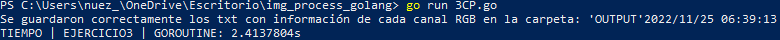
\includegraphics[scale=0.75]{CON3.png}
\end{figure}
\\
- SECUENCIAL: EJECUCIÓN Y TIEMPO EN CONSOLA (ADMIN/POWERSHELL):
\begin{figure}[h]
\centering
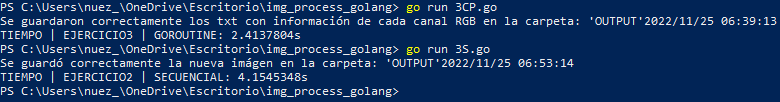
\includegraphics[scale=0.75]{SEC3.png}
\end{figure}
\\
- INPUT DE IMÁGEN (ARCHIVO: "ASTROWORLD"):
\begin{figure}[h]
\centering
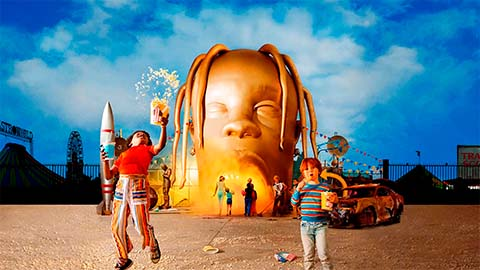
\includegraphics[scale=0.60]{ASTROWORLD.jpg}
\end{figure}
- OUTPUT DE IMAGEN RESULTANTE (se utilizó "Pandas", librería de python para graficar los histogramas):
\begin{figure}[h]
\centering
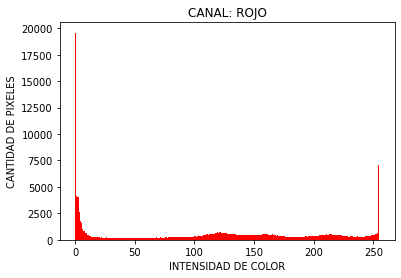
\includegraphics[scale=0.5]{red-gram.png}
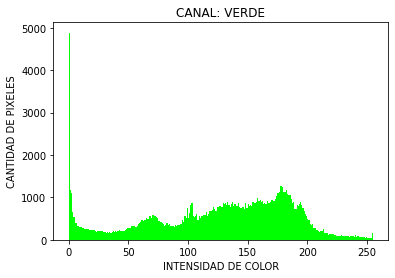
\includegraphics[scale=0.5]{green-gram.png}
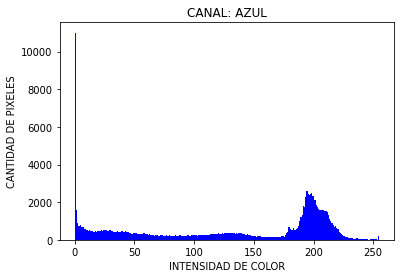
\includegraphics[scale=0.5]{blue-gram.png}
\end{figure}
\newpage
\section{CONCLUSIONES}
- GOLANG ES UN LENGUAJE CON EL QUE SE PUEDEN REALIZAR MÚLTIPLES FUNCIONES DE MANERA SENCILLA, ENTRE ELLAS ESTÁ PODER EDITAR IMÁGENES.
\\
- "GOROUTINES" VUELVE MÁS EFICIENTE LA EJECUCIÓN DE FUNCIONES;PUES HACE USO DEL PARALELISMO, PERMITIENDO QUE NUESTRO CÓDIGO SEA MÁS VELOZ EN CUANTO A TIEMPO DE EJECUCIÓN.
\\
- TENER EN CUENTA LA POTENCIA DEL PROCESADOR DEL EQUIPO CON EL QUE SE ESTÉ TRABAJANDO; NO EXCEDER LA CANTIDAD DE THREADS QUE SE ESTIMA; Y TENER EN CUENTA LOS POSIBLES FALLOS POR DEADLOCK.
\\
\newpage
\centering
GITHUB \href{https://github.com/ChristianRodriguez3012/FLP-IMAGENES_EN_GO}.
\end{document}
